\documentclass[a4paper,12pt]{article} 
\usepackage[T2A]{fontenc}			
\usepackage[utf8]{inputenc}			
\usepackage[english,russian]{babel}	
\usepackage{amsmath,amsfonts,amssymb,amsthm,mathrsfs,mathtools} 
\usepackage{cancel}
\usepackage{hhline}
\usepackage{multirow}
\usepackage[colorlinks, linkcolor = purple, citecolor = purple]{hyperref}
\usepackage{upgreek}\usepackage[left=2cm,right=2cm,top=2cm,bottom=3cm,bindingoffset=0cm]{geometry}
\usepackage{tikz}
\usepackage{graphicx}
\graphicspath{ {./pictures/} }
\usepackage{subfig}
\usepackage{titletoc}
\usepackage{tikz}
\usepackage{pgfplots}
\usepackage{xcolor}
\usepackage{wrapfig}
\usepackage{todonotes}

\newcommand\myworries[1]{\colorbox{red!30}{TODO #1}}
\newcommand\attention[1]{\colorbox{cyan!30}{#1}}

\title{Sem10Synopsis}
\begin{document}

\author{Александр Мишин, Б01-008а}
\date{}
\maketitle

\section*{МНК}

$$(\varphi_k, \varphi_j) = \sum_{i=0}^{n} x_i^{k + j}$$
$$f_k = \sum_{i = 0}^n y_i x_i^k$$

\begin{table}[h!]
\centering
\begin{tabular}{|l|r|r|r|r|r|}
\hline
x & -1 & -0,4 & 0 & 0,5 & 1    \\ \hline
y & -2 & -1   & 0 & 1,2 & 2,05 \\ \hline
\end{tabular}
\end{table}

$B \overrightarrow{a} = \overrightarrow{c}$

     \overrightarrow{B} = \begin{bmatrix}
       $(\varphi_0, \varphi_0)$ & $(\varphi_0, \varphi_1)$ & $(\varphi_0, \varphi_2)$ \\[0.3em]
       $(\varphi_1, \varphi_0)$ & $(\varphi_1, \varphi_1)$ & $(\varphi_1, \varphi_2)$ \\[0.3em]
        $(\varphi_2, \varphi_0)$ & $(\varphi_2, \varphi_1)$ & $(\varphi_2, \varphi_2)$ \\[0.3em]
    \end{bmatrix} \hspace{1cm}

$\varphi_0 = 1$, $\varphi_1 = x$, $\varphi_2 = x^2$\\

$(\varphi_0, \varphi_0) = \sum_{i=0}^4 1 = 5$\\

$c_0 = f_0 = \sum_{i=0}^4 y_i \cdot 1 = 0.25$\\

$(\varphi_0, \varphi_1) = \sum_{i=0}^4 x_i = 0.1$\\

$c_1 = f_1 = \sum_{i=0}^{4} y_i x_i^2 = (2 + 0.4 + 2.6 + 2.05) = 5.05$

     \overrightarrow{B} = \begin{bmatrix}
       5 & 0.1 & 2.41 \\[0.3em]
       0.1 & 2.41 & 0.061 \\[0.3em]
       2.41 & 0.61 & 9.0881 \\[0.3em]
    \end{bmatrix} \hspace{1cm}

    \overrightarrow{c} = \begin{bmatrix}
       0.25\\[0.3em]
       5.05\\[0.3em]
       0.19\\[0.3em]
    \end{bmatrix} \hspace{1cm}
    
Тогда получим полином\\
$P_2(x) = -0.01410 + 2.03485x + 0,0460x^2$

\subsection*{Пример 1}

$P_2(x) = ax^2 + b$

$\left\{\varphi_k\right\} = {{1; x^2}}$

Найти a, b:\\

[-1; 1] к f(x) = |x|

$B \overrightarrow{a} = \overrightarrow{c}$

\[(\varphi_0, \varphi_0) = \int_{-1}^1 1 \cdot 1 dx = 2\]
\[(\varphi_1, \varphi_0) = \int_{-1}^1 x^2 \cdot 1 dx = \frac{2}{3}\]
\[(\varphi_1, \varphi_1) = \int_{-1}^1 x^2 \cdot x^2 dx = \frac{2}{5}\]

\[c_1 = \int_{-1}^1 |x| \cdot x^2 dx = \frac{1}{2}\]
\[c_0 = \int_{-1}^1 |x| \cdot 1 dx = 1\]

    \begin{bmatrix}
       2 & 2/3\\[0.3em]
       2/3 & 2/5\\[0.3em]
    \end{bmatrix}
    \cdot
    \begin{bmatrix}
       a\\[0.3em]
       b\\[0.3em]
    \end{bmatrix}
    =
    \begin{bmatrix}
       1\\[0.3em]
       1/2\\[0.3em]
    \end{bmatrix}
    
Тогда получим b = 3/16, a = 15/16.

\subsection*{Пример 2}
\[P_1 = a_1 x + a_0\]

\begin{cases}
x + y  = 1  \\
2x + y = 2 \\
x + 2y = 3 \\
\end{cases}\\

$$Ax = f \xrightarrow{} A^T A \overrightarrow{x} = A^T \overrightarrow{f}$$
х - элемент  наилучш. среднеквадрат.

    f = \begin{bmatrix}
       1\\
       2\\
       3\\
    \end{bmatrix}\\
    A = \begin{bmatrix}
       1 & 1\\[0.3em]
       2 & 1\\[0.3em]
       1 & 2\\[0.3em]
    \end{bmatrix}\\
    $A^T$ = \begin{bmatrix}
       1 & 2 & 1\\[0.3em]
       1 & 1 & 2\\[0.3em]
    \end{bmatrix}\\
    $A^T A$ \cdot
    \begin{bmatrix}
       x\\
       y\\
    \end{bmatrix} 
    = \begin{bmatrix}
       6 & 5 \\[0.3em]
       5 & 6 \\[0.3em]
    \end{bmatrix}
    \cdot
    \begin{bmatrix}
       x\\
       y\\
    \end{bmatrix}
    =
    $A^T f$ = \begin{bmatrix}
       8 \\[0.3em]
       9 \\[0.3em]
    \end{bmatrix}\\

    Всегда следует проверять \det B \neq 0.\\
    
    Получим ответ x = 3/11, y = 14/11

\subsection*{Пример 3}

$$\int_{x_0}^{x_n} f(x) dx$$

Хочу привести численное интегрирование. \\

\attention{Формула Ньютона-Котеса}\\
Вспоминаем, что $f(x) = P_m(x) + R_m(x)$
Самое первое, чем можно заменить $P_m(x)$.

\section*{ Метод левых прямоугольников}

        \begin{figure}[h!]
            \centering
            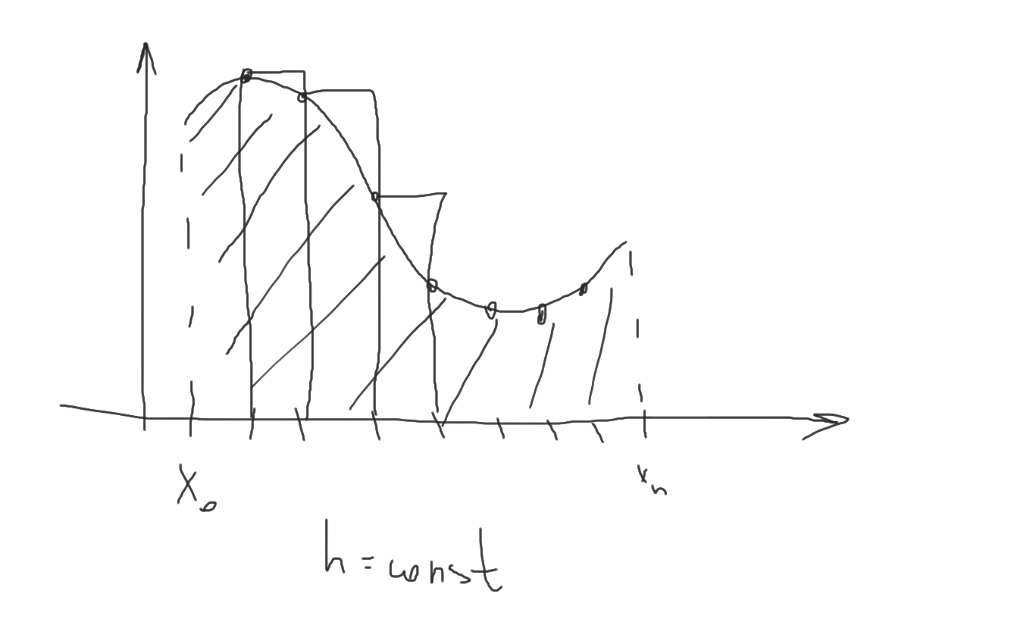
\includegraphics[width=8cm]{10SemPic1.png}
            \label{fig:vac}
        \end{figure}

$$\int_{x_0}^{x_n} f(x) dx \approx h \sum_{i = 0}^{n-1}f_i$$
$$|R(f)| \leq \max_{[x0, x_n]} |f'(x)| \frac{(x_n - x_0) \cdot h}{2}$$

\section* {Метод трапеции}

        \begin{figure}[h!]
            \centering
            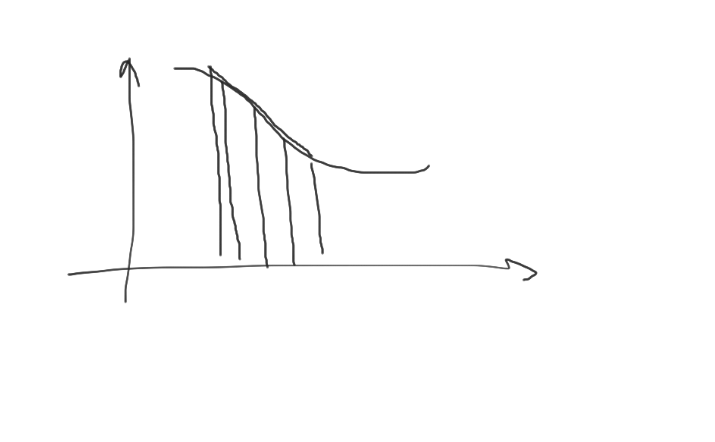
\includegraphics[width=8cm]{10SemPic2.png}
            \label{fig:vac}
        \end{figure}

$$\int_{x_0}^{x_n} f(x) dx \approx h [\frac{f_0 + f_n}{2} \sum_{i = 0}^{n-1}f_i]$$
$$|R(f)| \leq \max_{[x0, x_n]} |f''(x)| \frac{(x_n - x_0) \cdot h^2}{12}$$

\section* {Метод средних прямоугольников}
$$\int_{x_0}^{x_n} f(x) dx \approx h \sum_{i = 0}^{n-1}f(x_i - 1/2)$$
$$|R(f)| \leq \max_{[x0, x_n]} |f''(x)| \frac{(x_n - x_0) \cdot h^2}{24}$$

\section* {Формула Симпсона}

$$\int f(x) dx \approx \frac{h}{3} [f_0 + f_n + 4\cdot \sum_{i=1}{n/2} f_{2i-1} + 2 \sum_{i=1}^{n/2 - 1} f_2i]$$
n - чётное число

$$|R(f)| \leq \max_{[x_0, x_n]} |f^{(4)}| \frac{x_n - x_0}{180} \cdot h^4$$

\subsection*{Пример 4}
    (Для сравнения методов)\\
    $$\varepsilon \leq 10^{-2}$$
    
    \[I = \int_{-1}^1 \frac{x}{\sqrt{3}} \arctg (\frac{x}{\sqrt{3}}) dx\]
    промежуточно вычислим $M_2$ = 2/3

    \[\Delta I = \frac{M_2 h^2 (1 -(-1))}{12} = \frac{M_2 h^2 }{6} \leq \varepsilon\]

    \[h \leq 0.3\]
    \[h = \frac{x_n - x_0}{n} \overrightarrow{} n = [\frac{2}{0.3}] + 1 = 7\]
    
    \[I = \frac{M_4 h^4}{30} \leq \varepsilon\]
    $M_4 = 3/10$\\
    $h \leq 1.48$
    \[n = [\frac{2}{1.48}] + 1 = 2\]


\end{document}
